\chapter{Experimental observation of k/-k correlations in the depletion of a weakly-interacting Bose gas}

The Bogoliubov interacting Bose-gas has been the subject of a large variety of experimental studies (CITATIONS). However, these experiments have mainly focused on measuring the Bogoliubov spectrum of excitations. More than 60 years after the seminal Lee, Huang and Yang paper \cite{lee1957}, an experimental study of the correlations in the many-body ground-state is yet to be done. As we have seen thus far, our experimental setup is perfectly suited for such an investigation. 

The focus of this chapter will be on the experimental measurement of \kmk correlations in the depletion of a weakly-interacting Bose-gas. We will first detail the numerical procedure to compute two-body correlations from the measured momentum distributions \NOTE{FINIR}

W will analyze the results in the light of the theoretical predictions developed in Chapter 3. 

\section{Numerical procedure to measure two-body correlations}

\label{sec:numerical_calculation}

Our goal is to compute the normalized second-order correlation function:

\begin{equation}
    g^{(2)} (\bm{k},\bm{k'}) = \frac{\mean{\hat{a}^{\dagger}(\bm{k}) \hat{a}^{\dagger}(\bm{k'}) \hat{a}(\bm{k}) \hat{a}(\bm{k'})}}{\mean{\hat{a}^{\dagger}(\bm{k}) \hat{a}(\bm{k}) } \mean{\hat{a}^{\dagger}(\bm{k'}) \hat{a}(\bm{k'}) }}
\end{equation}

\noindent We recognize that $\mean{\hat{a}^{\dagger}(\bm{k}) \hat{a}(\bm{k})}$ is the momentum density in mode $\bm{k}$ that we will write $\rho(\bm{k})$ in the following. We remind to begin the result of chapter 1 which is that the $\gtwo$ function will take values different from 1 in two cases:

\begin{itemize}
    \item For $\bm{k'} \simeq \bm{k}$, the \textbf{normal} correlations corresponding to the Hanbury Brown and Twiss effect also known as bosonic bunching.
    \item For $\bm{k'} \simeq -\bm{k}$, the \textbf{anomalous} correlations corresponding to the \kmk pairs in the quantum depletion.
\end{itemize}

In practice, plotting the $\gtwo$ function defined as such does not make much sense. On the one hand, the function here is 6D and thus hard to plot in an intelligible way. On the other hand, obtaining a sufficient signal to noise ratio to make correlation measurements for single values of $\bm{k}$ and $\bm{k'}$ is impossible. The idea is then to integrate the $\gtwo$ function over all momenta $\bm{k}$ and introduce a new parameter $\delta \bm{k}$ to write:

\begin{equation}
    g_{N,A}^{(2)} (\delta {\bm k})=\frac{\int_{\Omega_{k}} \langle \hat{a}^{\dagger}({\bm k}) \hat{a}^{\dagger}(\delta {\bm k} \pm {\bm k}) \hat{a}({\bm k}) \hat{a}(\delta {\bm k} \pm {\bm k}) \rangle \mathrm{d}{\bm k}}{\int_{\Omega_{k}} \rho({\bm k}) \rho(\delta {\bm k} \pm {\bm k}) \mathrm{d}\bm{k}}
    \label{Eq:g2}
\end{equation}

\noindent With this definition, we see that for $\delta \bm{k}=\bm{0}$, we are either looking at \textbf{normal} \kk correlations (subscript N) when chosing the plus sign, or \textbf{anomalous} \kmk correlations (subscript A) with the minus sign. Note that we will often use the subscript $(N,A)$ for all definitions concerning both normal and anomalous correlation functions. We reduced the 6D function to a 3D function of the parameter $\delta \bm{k}$ which equals $\bm{0}$ when the correlation condition $\bm{k'} = \pm \bm{k}$ is fulfilled. This gives us a natural way to evaluate $\gtwo (\delta \bm{k})$ with the experimental data: we compute the values of the parameter $\delta \bm{k}$ for every detected atom pairs in an experimental run by calculating their momentum difference or sum for normal and anomalous correlations respectively. By computing the histogram of these values and averaging over many experimental runs, we evaluate the numerator of equation \ref{Eq:g2}.

\subsection{Description of the algorithm}

The algorithm described here is similar to the one used in our previous work \cite{carcy2019momentum,cayla2020} and detailed in \cite{cayla_these,carcy_these}. This previous version was mainly designed for the observation of bosonic bunching. I adapted the algorithm to make it suitable for the calculation of \kmk correlations as well, as we will discuss now.

\subsubsection{Numerator calculation}

The first step is to compute the numerator of equation \ref{Eq:g2} that we denote $G^{(2)}(\delta \bm{k})$. We note $N_{runs}$ the number of experimental runs and $N_{i}$ the number of atoms in the $i$-th shot. The procedure is as follows:

% \begin{algorithm}
% \caption{$G^{(2)}$ calculation}
%     \begin{algorithmic}{}
%         \FOR{$i=1:N_{runs}$}
%             \FOR{$j=1:N_{i}$}
%                 \STATE Compute $\vec{k}_i+\vec{k}_j$
%                 \STATE Increment histogram $G^{(2)}$ corresponding pixel
%             \ENDFOR
%         \ENDFOR
%     \end{algorithmic}{}
% \end{algorithm}

\begin{algorithm}
 \caption{$G^{(2)}$ calculation}
    \begin{algorithmic}
         \For{$i=1:N_{runs}$}
            \For{$j=1:N_{i}$}
               \For{$p=1:N_{i}$}
                    \State Compute $\delta \bm{k} = \bm{k}_j \pm \bm{k}_p$
                    \State Increment 3D histogram $G^{(2)}$ corresponding voxel
                \EndFor
            \EndFor
        \EndFor
\end{algorithmic}

\end{algorithm}

We end up with a 3D histogram where each voxel is associated to a value of $\delta \bm{k} = (\delta k_x,\delta k_y, \delta k_z)$ and records how many atom pairs have this specific momentum sum or difference, depending on the kind of the correlations we want to probe.

The major difference with the previous version of the algorithm is that we record here the full 3D histogram of calculated $\delta \bm{k}$ on every pair of atoms. The procedure was originally made simpler by calculating three one-dimensional histograms, one for each direction of space. Each of these histograms represents a one-dimensional cut in the general 3D histogram $G^{(2)}(\delta \bm{k})$. For instance, the $x$ direction histogram was obtained by selecting one atom labelled $i$ and calculating $\delta k_x$ only for atoms close in momentum space, \ie with $|k_y^{(i)}-k_y^{(j)}| \leq \Delta k_{\perp}$ and $|k_z^{(i)}-k_z^{(j)}| \leq \Delta k_{\perp}$, where $\Delta k_{\perp}$ defines a transverse integration (see later). This method obviously saves computing time and RAM space, but is not suited to look for \kmk correlations.

At this point, we record in the central voxels associated to $\delta \bm{k} \simeq \bm{0}$ what we call \textbf{true coincidences}, namely two atoms detected conjointly as a result of \kmk pairing or bosonic bunching. However, we also record \textbf{accidental coincidences} that do not represent correlations but result from the distribution of the atoms. We then need a normalization process to get rid of the contribution of accidental coincidences. 

\subsubsection{Denominator calculation}

\label{sec:algo}

We now want to compute the denominator of equation \ref{Eq:g2}, representing the effect of accidental coincidences. To perform this calculation, we would like to have a sample of atoms with the same momentum density than our experimental data but uncorrelated. This can be done by merging all experimental shots, not correlated with one another. We then apply the procedure we have just described to this data set. However, some of the correlations happening in single shots will remain in this large file. In the end, the total number of correlations in the numerator is $\sum_i N_i^2$ whereas the number of coincidences in the merged file is $(\sum_i N_i)^2$. If we note $\bar{N}$ the mean number of atoms per shot, we see that :

\begin{equation}
      \frac{\sum_i N_i^2}{(\sum_i N_i)^2}=\frac{N_{\rm{runs}} \bar{N}^2}{N_{\rm{runs}}^2 \bar{N}^2}=\frac{1}{N_{\rm{runs}}}
\end{equation}{}

Therefore, with enough shots, the contribution of residual coincidences in the denominator is negligible. 

In the end, the integrated $g^{(2)}$ function can obtained by dividing the calculated numerator by the denominator and multiplying by the normalization factor $\frac{(\sum_i N_i)^2}{\sum_i N_i^2}$ taking into account the number of coincidences of the numerator and denominator. It is possible to take a fraction of all atoms for the denominator calculation to avoid large computation time. This is particularly handy to have quick first results before launching longer calculations for a nicer signal-to-noise ratio.

\subsection{Accessing the BEC depletion}
\label{sec:accessing_depletion}

In order to detect \kmk pairs in the depletion, it is absolutely crucial to remove from the analysis all atoms belonging to the BEC and its diffracted copies showing no correlations as it is a pure coherent state. These atoms indeed largely outnumber the depleted atoms and will therefore entirely drown out the \kmk correlation signal of the quantum depletion, would they not be removed. 
For each recorded data set and before running the algorithm, we remove all atoms outside the volume $\Omega_k$ that we design to exclude momentum regions with condensed atoms as illustrated on Fig-\ref{fig:omega_k}. We set $\Omega_k$ to have a cubic symmetry that matches the symmetry of the momentum distribution in a cubic lattice. We remove all atoms with $|k_i| < k_{\rm{min}}$ and $|k_i| > k_{\rm{max}}$ where $k_i$ is the momentum projection along an axis $i=x,y,z$. We use $k_{\rm{min}}=0.15 \, k_d$, corresponding to $\sim 6$ times the RMS width of the BEC peaks, in order to ensure that all condensed atoms have been removed. The high limit is set to $k_{\rm{max}}=0.85 \, k_d$ to exclude higher order peaks and is slightly smaller than the momentum range probed by the MCP.

\begin{figure}
    \centering
    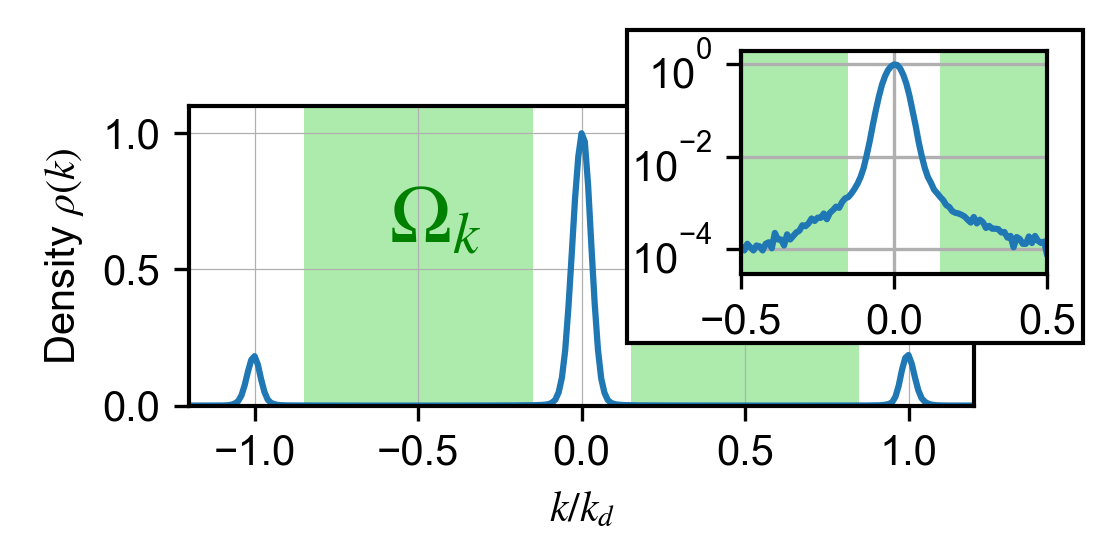
\includegraphics[width=0.8\textwidth]{Fig/Chapter4/densite.png}
    \caption{1D cut of the momentum density illustrating the integration volume $\Omega_k$. The central peak corresponds to the BEC and the lateral peaks at $\pm \ k_d$ to diffraction peaks induced by the presence of the optical lattice. The green area shows the volume $\Omega_k$ containing the depleted atoms selected for the correlation measurement. While barely visible in linear scale, they can be seen in the log scale plot shown in inset.}
    \label{fig:omega_k}
\end{figure}


\subsection{Benchmarking of the algorithm with two-body collision spheres}

Before using the algorithm to look for a supposedly small \kmk pairing signal in the depletion of a weakly-interacting Bose gas, it was crucial to test it on a data set with a large number of \kmk pairs to certify that it was working properly. Luckily, we could re-use the data taken for measuring two-body collisions during the time-of flight described in Chapter 2. The simplest case is to use only one of the lattice beam to induce 1D diffraction and observe only two collision spheres. \NOTE{FINIR}




\section{Observation of the pair correlation signal}

\subsection{Experimental parameters}
\label{sec:post_selec}

We prepare a BEC with a target number of $\NBEC=5 \times 10^3$ atoms in an optical lattice of amplitude $V=7.75 \ E_r$. With this lattice amplitude, we are in the superfluid domain of the phase diagram in which we expect the \kmk correlations. In order to have sufficient statistics, we repeat the experiment $\sim 4,000$ times. In practice, we cannot prepare BECs with the exact same number of atoms at each shot. We then need to post-select the data and remove runs with a detected atom number falling too far from the target number. We allow for $30 \%$ fluctuations around the target number and end up conserving around $\sim 2,000$ runs.

\subsection{$g^{(2)}_A$ correlation function}

We have plotted on Fig-\ref{fig:kmk_signal} 1D cuts through the $g_{A}^{(2)}$ function on which we can see clear correlation peaks standing out from the noise! The peaks are well-fitted with a Gaussian function (\NOTE{COMPLETER}). At this point, we must stress out that the novelty of this signal is that it is the first experimental observation of \kmk pairs in an \textbf{at-equilibrium system}. They have indeed been numerous observations of \kmk pairs, but always in \textbf{out-of-equilibrium} configurations. To a cite a few examples:

\begin{itemize}
    \item Parametric down conversion in quantum optics \cite{burnham1970}.
    \item Dissociation of diatomic molecules in atomic physics \cite{greiner2005}.
    \item Elastic collisions in high energy physics \cite{arnison1982} or with ultracold atoms \cite{perrin2007observation}.
\end{itemize}

\begin{figure}
    \centering
    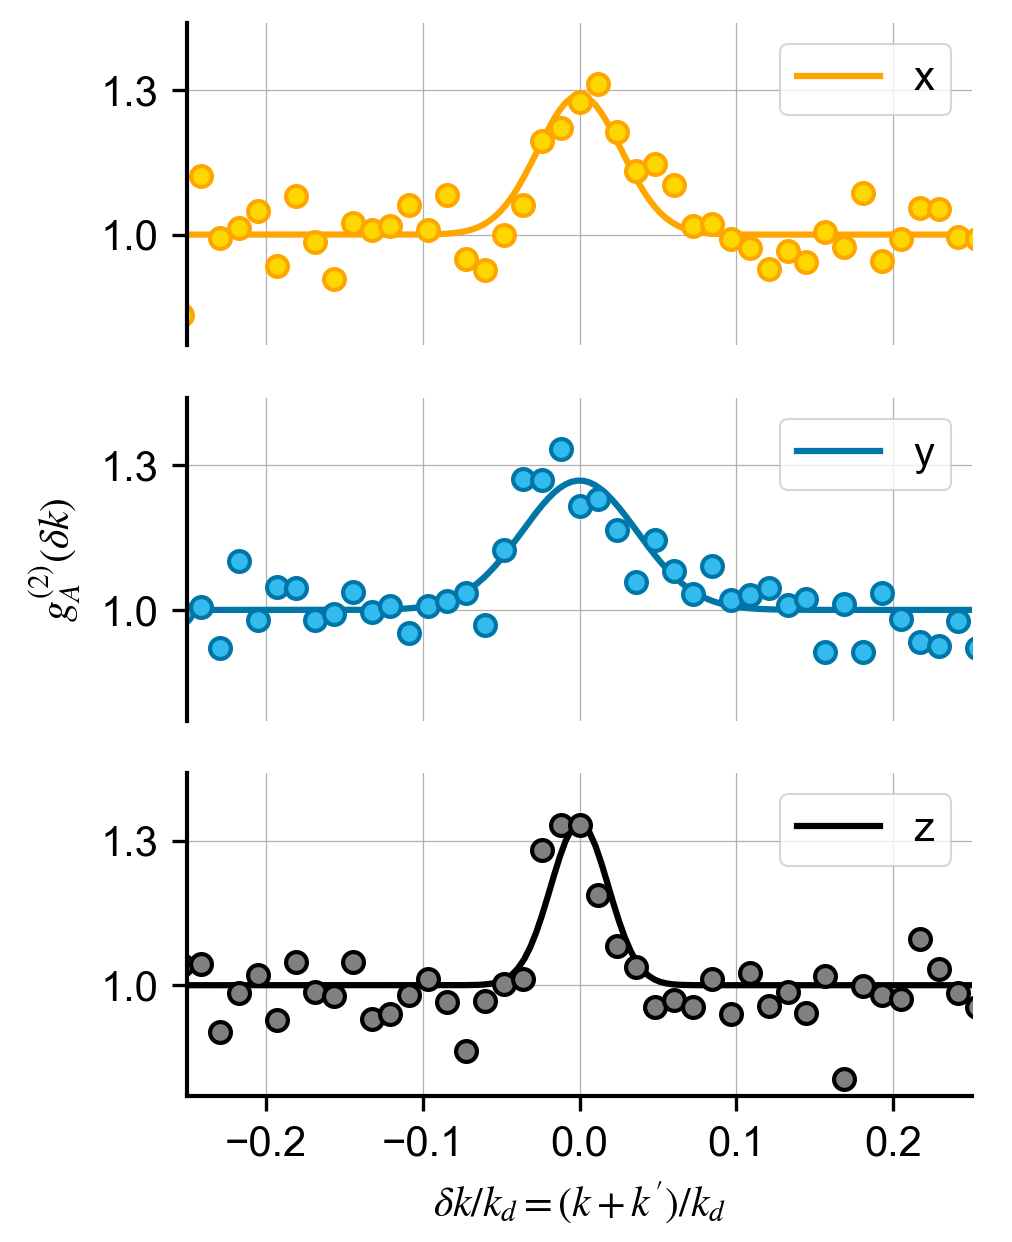
\includegraphics[width=0.65\textwidth]{Fig/Chapter4/1d_cuts.png}
    \caption{1D cuts through $g_{A}^{(2)} (\delta {\bm k})$ along the axis of the 3D optical lattice. The transverse integration is $\Delta k_{\perp}=3 \times 10^{-2} \ k_d$ and the longitudinal pixel size is $\Delta k_{\parallel}=1.2 \times 10^{-2} \ k_d$. The data is fitted by Gaussian functions (solid lines). The nice correlation peaks signal the presence of \kmk pairs.}
    \label{fig:kmk_signal}
\end{figure}

\noindent As we have discussed in Chapter 1, the \kmk pairs present in an at-rest BEC and are predicted to be populated through the interplay between interactions and quantum fluctuations for which we cannot draw any classical picture. Now that we have the experimental \kmk correlation signal, we can look to characterize it and determine whether our observations match what is expected from Bogoliubov theory and get a ``smoking gun'' argument that we are indeed seeing the \kmk correlations of the quantum depletion. In a first time, we will take a look at the effect of temperature that is supposed to destroy the \kmk correlation signal that reveals $T=0$ quantum coherences as explained in Chapter 1.

\section{Effect of temperature}

The temperature can be increased in a rather simple manner by holding the atoms at the final amplitude of the lattice for a longer duration, the gas being continuously heated over time (attributed to imperfections such as spontaneous emission or mechanical vibrations). We repeat the experiment with a holding time of $500 \ \rm{ms}$ corresponding to hundreds of tunneling times $225 \times h/J$. The increase in temperature can be seen by looking at the momentum density profile as shown in the panel b of Fig-\ref{fig:kmk_temperature}. As expected, the thermal depletion has increased, increasing the momentum density in the depletion region by a factor 4. Note however that we did not increase the temperature too much to keep a significant condensed fraction of the order of $f_c = 29 \%$ not to entirely remove the quantum depletion. This increase of the thermal depletion implies a decrease of $\gtwo_A (\bm{0})$ of at least a factor $4^2$, bringing it under the experimental noise, as we see on Fig-\ref{fig:kmk_temperature} panel a.

We also repeated the experiment for an intermediate temperature obtained with a holding time of $200 \ \rm{ms}$ corresponding to $90 \times h/J$ tunneling time. The condensed fraction is then $f_c=55 \%$ and we observe, as expected, a peak of intermediate amplitude as shown on Fig-\ref{fig:kmk_3_temp}.

\begin{figure}
    \centering
    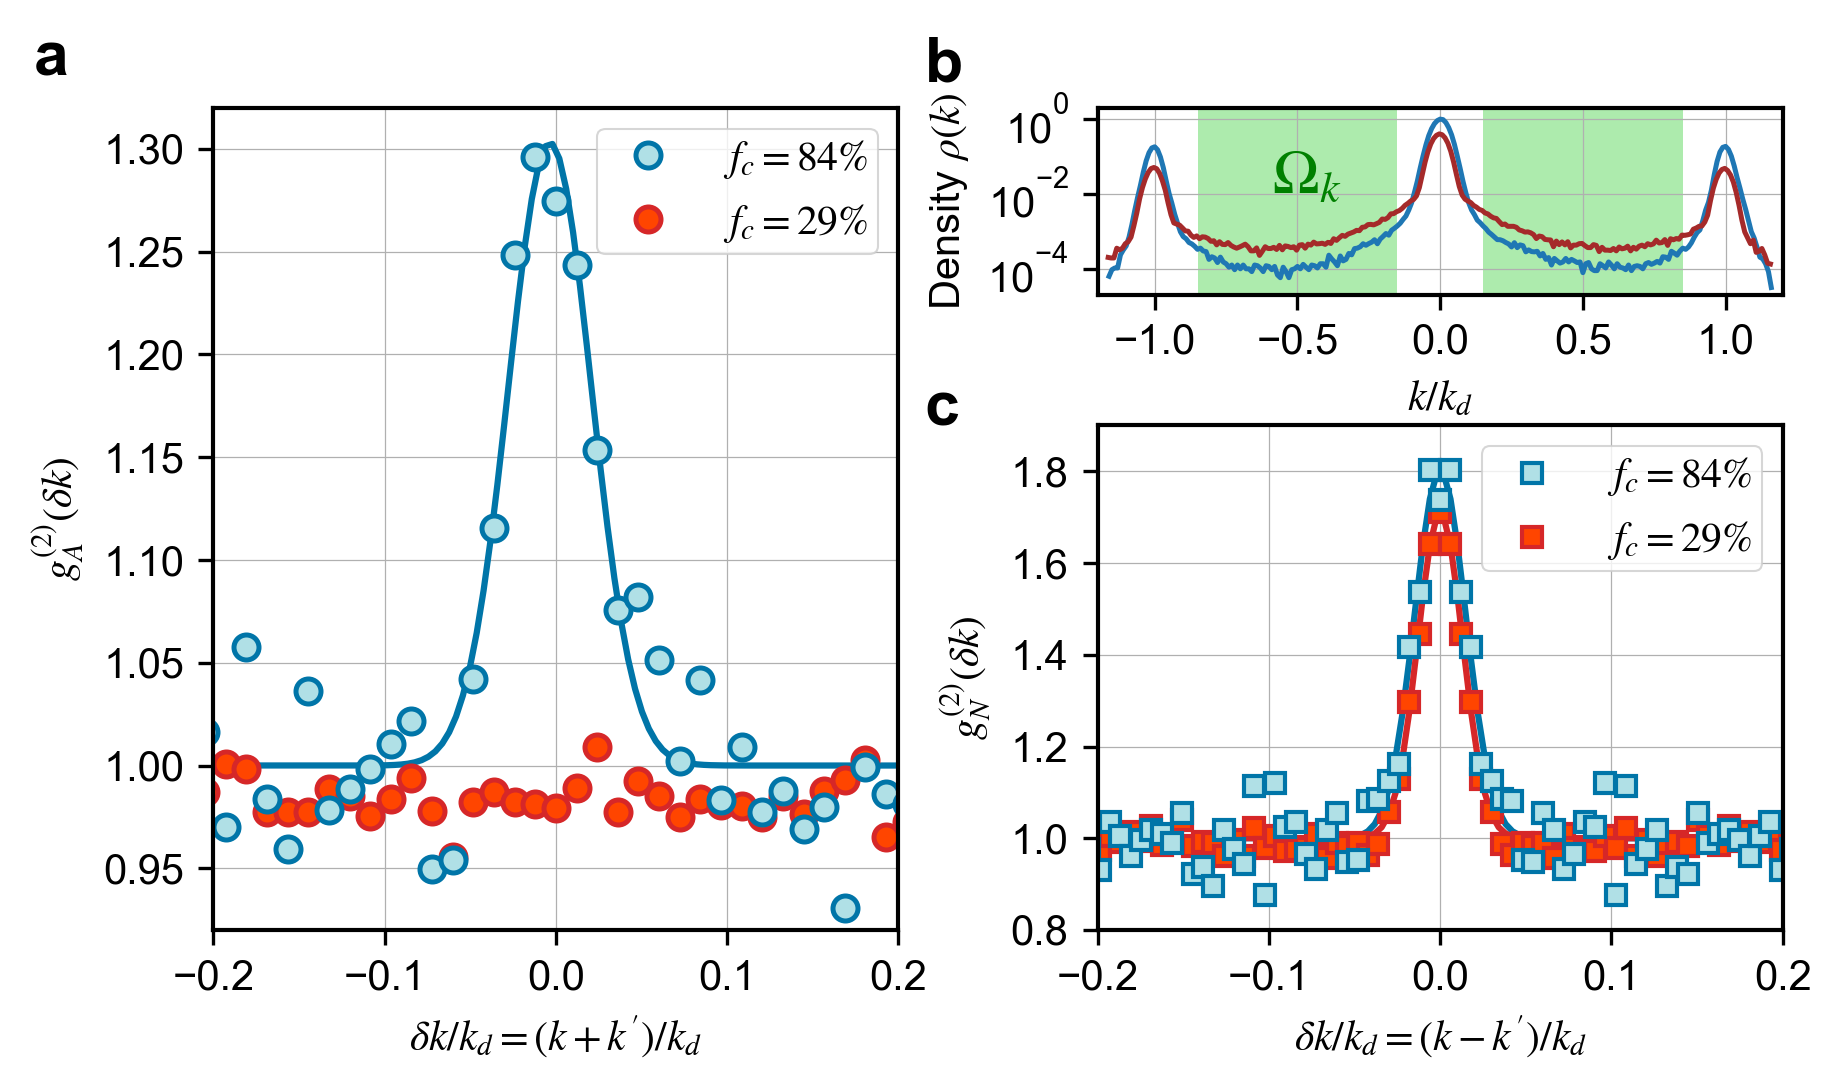
\includegraphics[width=\textwidth]{Fig/Chapter4/kmk_temperature.png}
    \caption{Atom-atom correlations in weakly-interacting BECs at two different temperatures. The data for the low-temperature BEC ($f_{c}=84\%$), {\it resp.} for the heated BEC ($f_{c}=29\%$), are depicted in blue, {\it resp.} in red. 
    {\bf (a)}. Anomalous correlations $g_{A}^{(2)}(\delta k)$ at opposite momenta. The ${\bm k}$/$-{\bm k}$ peak disappears as the temperature increases.
    {\bf (b)}. 1D cut of the density $\rho(k)$ in semilog scale. The depletion density increases with temperature.
    {\bf (c)}. Normal correlations $g_{N}^{(2)}(\delta k)$ for the same datasets and $\Omega_k$. The peak amplitude shows no significant change as the temperature increases. Note that the transverse integration $\Delta k_{\perp}=1.5 \times 10^{-2} \, k_d$ used here reduces the amplitude of the peaks.}
    \label{fig:kmk_temperature}
\end{figure}

We thus see that the \kmk correlation signal is extremely sensitive to temperature as predicted, hinting to the fact that it is indeed related to a $T=0$ ground-state effect. It is also quite illuminating to compare the \kmk correlations to the bosonic bunching \kk correlations. As explained in Chapter 1, the bosonic bunching effect is the consequence of chaotic statistics, a property shared by the thermal and quantum depletion. Therefore, changing the temperature and thus the balance between thermal and quantum depletion has no effect on bosonic bunching. This is what we observe experimentally as shown on Fig-\ref{fig:kmk_temperature} panel c.

In conclusion, we have on the same experimental data two very different behaviours with temperature that illustrate nicely the natures of the correlation signals. On the one hand, \kk correlations unaffected by temperature reveal the chaotic statistics of the system, on the other hand, \kmk correlations reveal the many-body ground state quantum coherences. These observations constitutes a rather convincing argument that we are indeed observing a \kmk correlation signal caused by the quantum depletion and not some other effect that we could have overlooked.

\begin{figure}
    \centering
    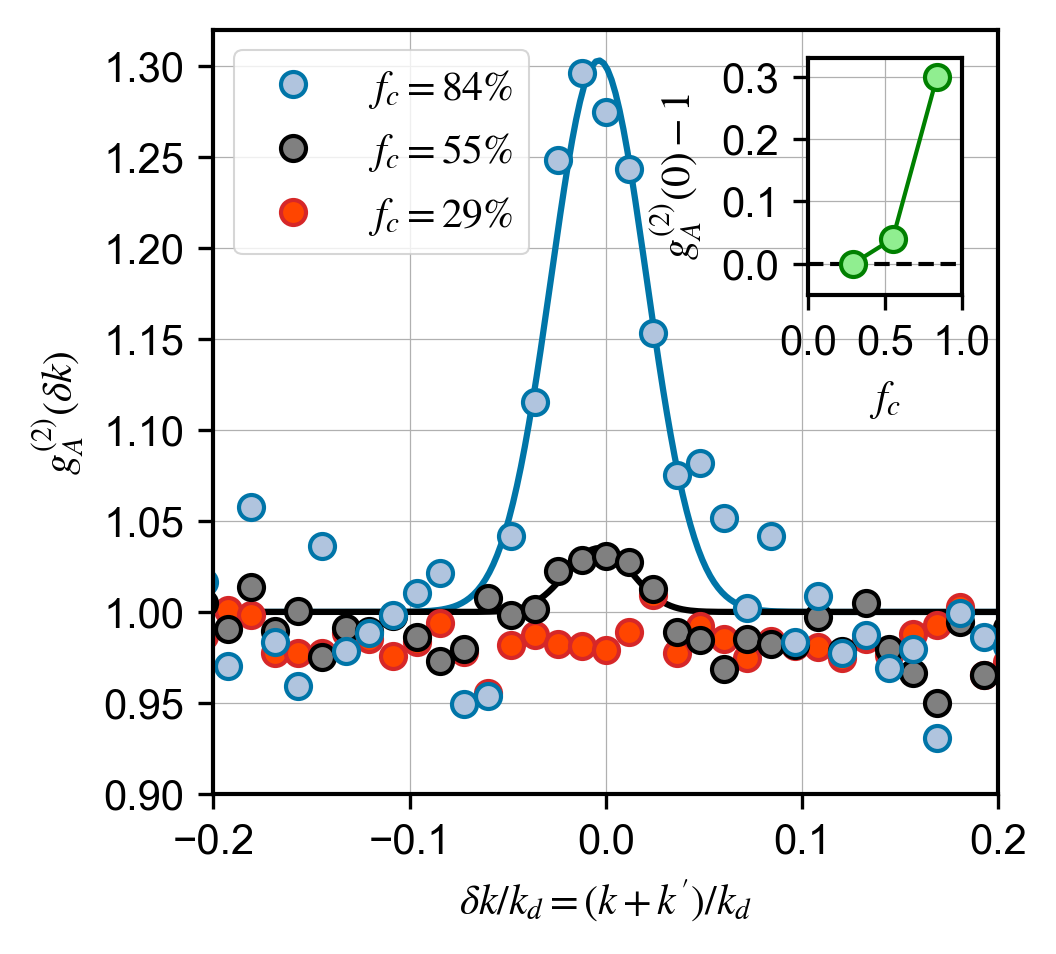
\includegraphics{Fig/Chapter4/kmk_3_temp.png}
    \caption{Anomalous correlation function for data sets with different temperatures and condensed fractions. The amplitude of the $\bm{k}$/$-\bm{k}$ correlation signal is progressively lost as the temperature rises and the condensed fraction diminishes. Inset: amplitude of the correlation peak $g^{(2}_{A}({\bm 0})$ as a function of the condensed fraction $f_c$.}
    \label{fig:kmk_3_temp}
\end{figure}



The attentive reader would have noticed than even though we expect perfect bosonic bunching $\gtwo_N (\bm{0})=2$, we rather observe $\gtwo_N (\bm{0}) \simeq 1.8$. This is due to transverse integration effects of the 3D $\gtwo$ function that we will now discuss.

\section{Study of the amplitude of the correlation peaks}

\subsection{Transverse integration effects}

The ``true'' theoretical, normalized and integrated two-body correlation function is modelled by a 3D Gaussian function:

\begin{equation}
    \gtwo (\delta \bm{k}) = 1 + \eta_0 \prod_{i=x,y,z} \exp \left(\frac{-\delta k_i^2}{2 \sigma_i}\right)
    \label{eq:g2_theo}
\end{equation}

\noindent where we introduce $\eta_0$ the amplitude of the correlation peak and $\sigma_i$ the RMS width of the correlation peak in direction $i=x,y,z$. Note that we will detail here a general calculation that applies for both normal and anomalous correlation.

As mentioned in \ref{sec:numerical_calculation}, the values of the $\gtwo$ function are recorded in a 3D histogram made of cubic voxels whose size will be denoted $\Delta k_{\parallel}$. To extract a 1D cut along $x$ direction for instance, we could simply take the line of voxels verifying $\delta k_y=\delta k_z =0$. However, this is often not sufficient to have a proper signal-to-noise ratio. We therefore rather average the values of several voxels lines associated to $\delta \bm{k}$ values verifying $\abs{\delta k_y, \delta k_z} \leq \Delta k_{\perp}$ as illustrated on Fig-\ref{fig:cube_integration}.

\begin{figure}
    \centering
    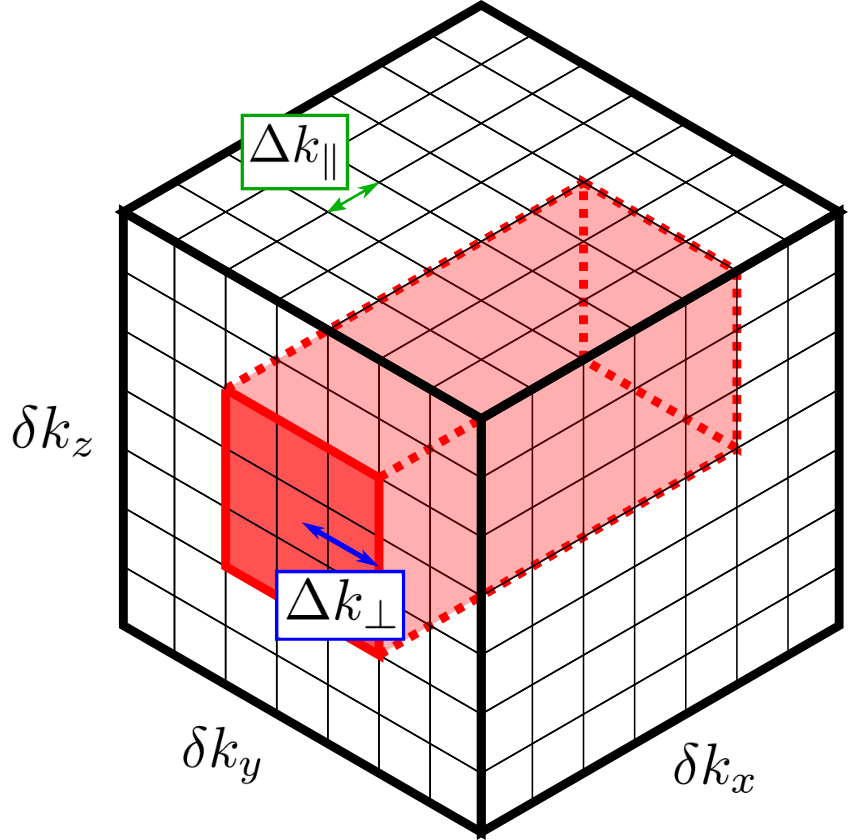
\includegraphics[width=0.45\textwidth]{Fig/Chapter4/cube_integration.png}
    \caption{Illustration of the transverse integration. Every voxel contains the value of the $\gtwo$ function for a given value of $\delta \bm{k}=(\delta k_x, \delta k_y, \delta k_z$). The figure illustrates the procedure to take a 1D cut in the $x$ direction: we average over several pixel lines to increase the signal-to-noise ratio. This is the transverse integration $\Delta k_{\perp}$ as defined on the schematic.}
    \label{fig:cube_integration}
\end{figure}

We can now re-write equation \ref{eq:g2_theo} to show what is the function that is actually plotted when taking a 1D cut along the $x$ direction after the transverse integration process:

\begin{equation}
    g^{(2)} \left(\delta k_{x}\right)=\frac{1}{\left(2 \Delta k_{\perp}\right)^{2}} \iint_{-\Delta k_{\perp}}^{\Delta k_{\perp}} \left( 1+ \eta_0 \prod_{i=x, y, z} \exp \left(\frac{-\delta k_{i}^{2}}{2 \sigma_i^{2}}\right) \rm{d} \delta k_y \rm{d} \delta k_z \right)
\end{equation}

This expression can be analytically evaluated and writes:

\begin{equation}
    g^{(2)} \left(\delta k_{x}\right)=1+\eta_0 \frac{2 \pi \sigma_y \sigma_z}{\left(2 \Delta k_{\perp}\right)^{2}} \exp \left(\frac{-\delta k_{x}^{2}}{2 \sigma_{z}^{2}}\right) \operatorname{erf}\left(\frac{\Delta k_{\perp}}{\sqrt{2} \sigma_{y}}\right) \operatorname{erf}\left(\frac{\Delta k_{\perp}}{\sqrt{2} \sigma_{z}}\right)
\end{equation}

Note that we have here neglected the small longitudinal integration induced by the size of the voxel, which is much smaller (\NOTE{CHIFFRES?}) than the typical width of the correlation peaks. In addition and as we will see later (\NOTE{A VERIFIER DANGEREUX}), we assume that the correlation peaks are isotropic giving $\sigma_x=\sigma_y=\sigma_z=\sigma$. We thus see that when measuring any correlation peak amplitude with a Gaussian fit on a 1D cut of the $\gtwo$ function, we get a reduced amplitude $\eta$ that writes:

\begin{equation}
    \eta (\Delta k_{\perp})= \eta_{0} \times \frac{2 \pi \sigma^2}{(2\Delta k_{\perp})^2}\left[\rm{erf} \left(\frac{\Delta k_{\perp}}{\sqrt{2}\sigma} \right)\right]^2
    \label{eq:fit_integration}
\end{equation}

The idea is then to measure $\eta$ for several values of $\Delta k_{\perp}$ and fit the data with equation \ref{eq:fit_integration} with $\eta_0$ and $\sigma$ as free parameters. For a single value of the transverse integration, $\eta$ is obtained by averaging the 3 amplitudes fitted on the 1D cuts along the 3 directions of space.


\NOTE{CHANGER} We show on Fig-\ref{fig:integration_kk} the results of this method applied to the bosonic bunching measurement for two temperatures as discussed in the previous section. 

\subsection{Normal correlations}

Coming back to the normal correlations plot of Fig-\ref{fig:kmk_temperature}, we now apply the method we have just described to correct the effects of the transverse integration with the results shown on Fig-\ref{fig:integration_kk}. From the fitted value of $\eta_{0,N}$, we obtain $g^{(2)}_N(\bm{0})=2.05(6)$ and $g^{(2)}_N(\bm{0})=2.09(5)$ for the high and low condensed fraction data sets respectively. These numbers are consistent with $\gtwo_N (\bm{0})=2$ expected for perfect bosonic bunching, confirming the prediction of the Bogoliubov theory. 

\begin{figure}
    \centering
    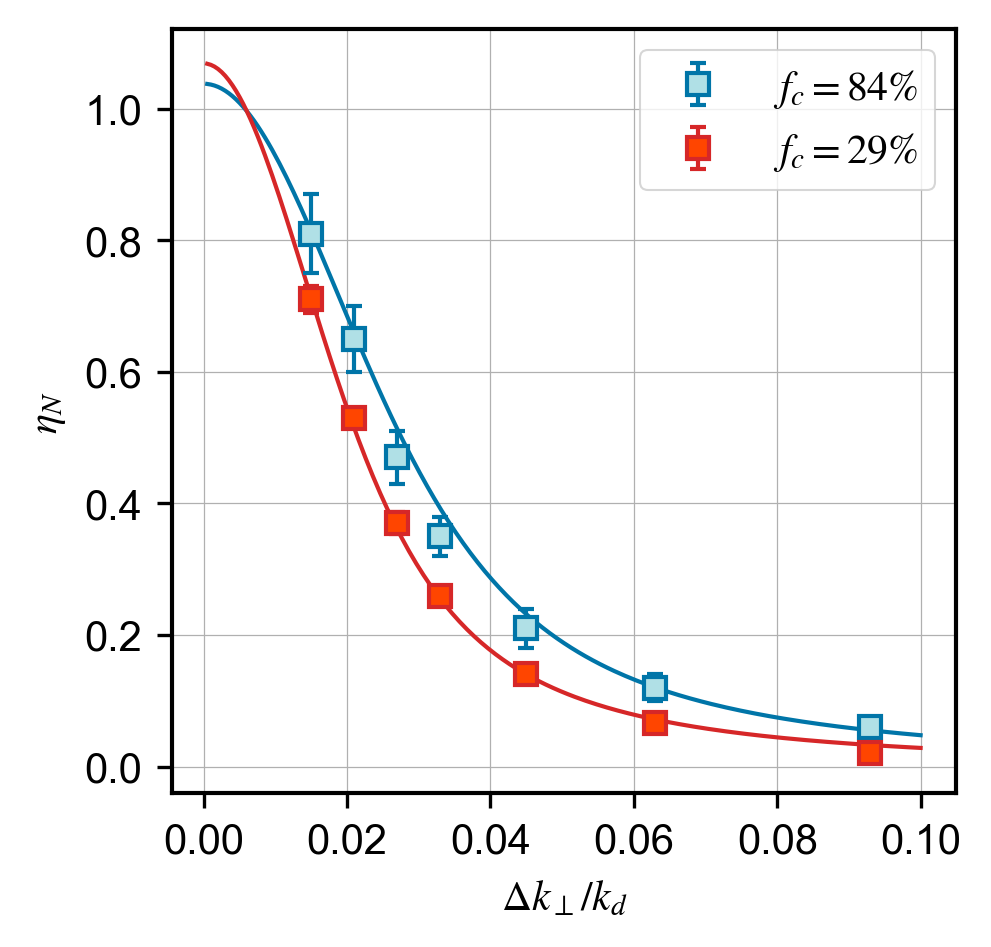
\includegraphics[width=0.65\textwidth]{Fig/Chapter4/eta_vs_int_kk.png}
    \caption{Fitted amplitude of the normal correlation peak $\eta_N$ as a function of the transverse integration $\Delta k_{\perp}$. The data is fitted with model defined in equation \ref{eq:fit_integration} with $\eta_0$ and $\sigma$ as free parameters. This method allows us to extract the amplitude at zero transverse integration $\eta_{0,N}$.}
    \label{fig:integration_kk}
\end{figure}

\subsection{Anomalous correlations}

We now turn to analyzing the amplitude of the anomalous correlation peaks. As we have seen with the calculations developed in section \NOTE{ADD SECTION NUMBER}, we can draw a clear analogy between the Bogoliubov weakly-interacting Bose gas and two-mode squeezed states in quantum optics. We showed that for such states, the amplitude of the anomalous correlation peak is expected to scale linearly with the inverse of what is called the average mode occupancy, {\it i.e.} the average number of photons per mode. In atomic physics, the analog to the average mode occupancy is the momentum density, {\it i.e.} the average number of atoms in a certain mode $\bm{k}$.

As explained in \ref{sec:accessing_depletion}, we measure integrated correlation functions over the momentum volume $\Omega_k$. The parameter setting the amplitude we observe is then the average momentum density $\bar{\rho}_{\Omega_k}$ defined as:

\begin{equation}
    \bar{\rho}_{\Omega_k}=\int_{\Omega_{k}} \rho({\bm k}) {\rm d}{\bm k}
\end{equation}

We have several possibilities to change the value of $\bar{\rho}_{\Omega_k}$:

\begin{itemize}
    \item Change the experimental parameters to load a different target total atom number $\NBEC$ in the optical lattice.
    \item "Artificially" change the total atom number $\NBEC$ by changing the target atom number when doing the data post-selection (see \ref{sec:post_selec}).
    \item Change the bounds of the integration volume $\Omega_k$.
\end{itemize}

We prepare 4 data sets using a combination of these 3 possibilities. We perform the experiment with a target loaded atom number $\NBEC=[2.5,5,10] \times 10^3$, and extract an additional set with $\NBEC=3.5 \times 10^3$ from the data intended for $\NBEC = 5 \times 10^3$ by changing the post-selection criterion. We also reduce $\Omega_k$ to momenta between $k_{\rm{min}} = 0.3 \ k_d$ and $k_{\rm{max}} = 0.7 \ k_d$, {\it i.e.} to a region where the depletion is lower. We thus reduce $\bar{\rho}_{\Omega_k}$ and observe higher amplitude values, a feature that we will use when interpreting the results later on.

The results are plotted on Fig.-\ref{fig:amplitude_vs_rhob} alongside the normal correlations amplitude for comparison. As expected, we observe a nice linear scaling of the anomalous amplitude with the inverse average density. On the other side, changing $1/\rhob$ does not change the chaotic nature of the system statistics, we thus observe $\gtwo_N (\bm{0})=2$ independently of the value of $\rhob$. Once again, the amplitudes were corrected of transverse integration effects as shown on Fig.-\ref{fig:eta_vs_int_kmk}

\begin{figure}
    \centering
    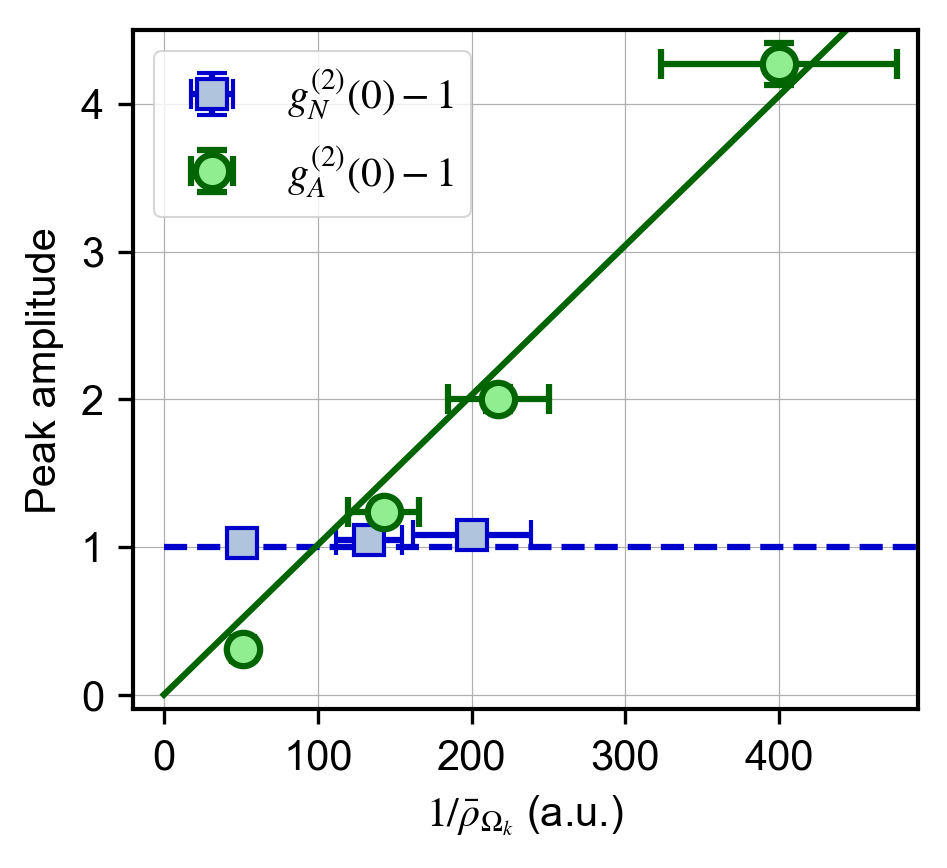
\includegraphics[width=0.65\textwidth]{Fig/Chapter4/amplitude_kmk.png}
    \caption{Amplitude of the correlation peaks versus the inverse average density $\rhob$. We observe a linear scaling for anomalous correlations, while normal correlations stay constant and compatible with $\gtwo_N (\bm{0})=2$.}
    \label{fig:amplitude_vs_rhob}
\end{figure}

\begin{figure}
    \centering
    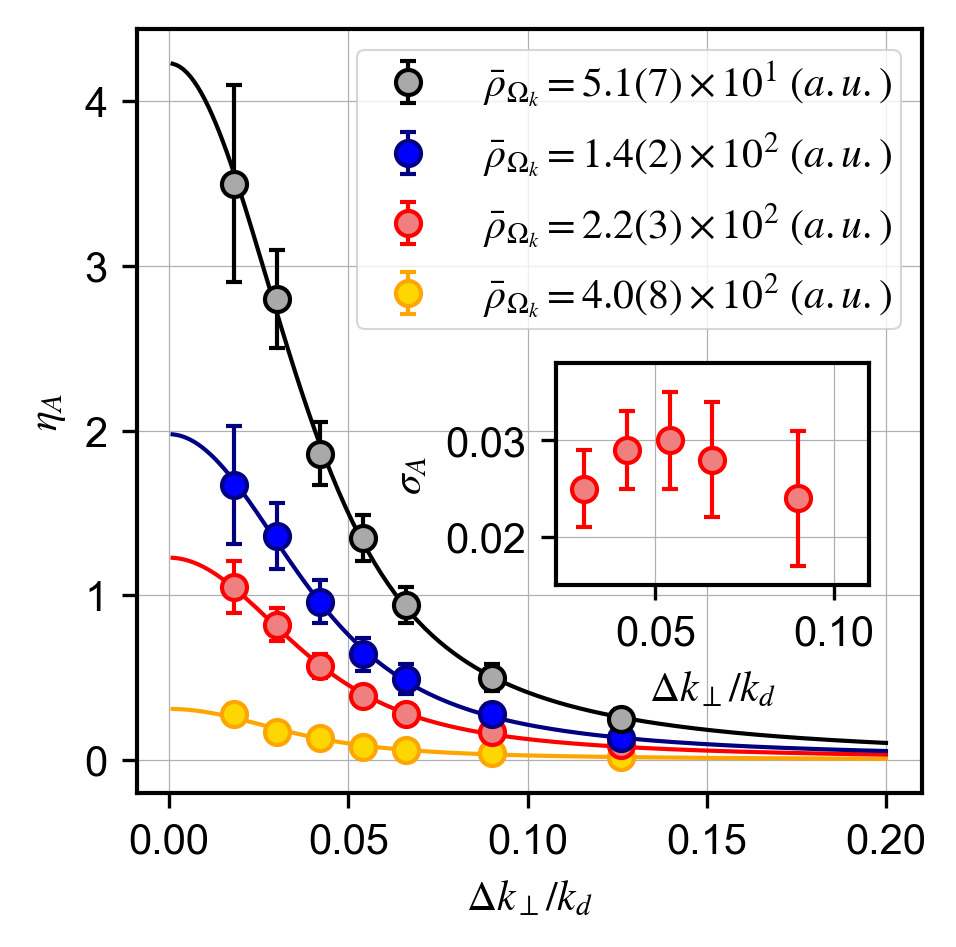
\includegraphics[width=0.65\textwidth]{Fig/Chapter4/eta_vs_int_kmk.png}
    \caption{Fitted amplitude of the normal correlation peak $\eta_N$ as a function of the transverse integration $\Delta k_{\perp}$.}
    \label{fig:eta_vs_int_kmk}
\end{figure}

\subsubsection{Discussion on the detected number of atom pairs}

After looking at the scaling of the amplitude, we take a look at the absolute value of the amplitude from which we extract the number of detected \kmk pairs. To this mean, the procedure is slightly changed:

\begin{enumerate}
    \item The voxel size is increased to $\Delta k_{\parallel} = 0.3 \ k_d$ so that the central voxel contains the entirety of the correlation peak.
    \item We count the number of coincidences $N_{\rm{numerator}}$ in the central voxel of the numerator of equation \ref{Eq:g2}. This number is the sum of the true coincidences caused by the \kmk pairs and accidental coincidences.
    \item  We count the number of coincidences $N_{\rm{denominator}}$ in the central voxel of the denominator to evaluate the number of accidental coincidences.
    \item We evaluate the number of atoms in a \kmk pair with $N_{\rm{pairs}}=N_{\rm{numerator}} - N_{\rm{denominator}} \times \frac{\sum_i N_i^2}{(\sum_i N_i)^2}$ where we recognize the normalization factor described in \ref{sec:algo}.
\end{enumerate}

When applying this procedure for the data set $\NBEC=5 \times 10^3$, $f_c=84 \%$, we find that we detect on average $0.5$ pairs per shot, for roughly $N_{\Omega_k}=100$ atoms detected in $\Omega_k$. We push the analysis a little further to calculate the fraction of quantum depleted atoms in the overall depletion condensate that we will write $\alpha_Q$. We first assume that all atoms in the quantum depletion form a \kmk pair and that atoms forming a \kmk pair necessarily belong to the quantum depletion. We then have:

\begin{equation}
    N_{\rm{pairs}}= N_{\Omega_k} \alpha_{\rm{MCP}} \alpha_Q
    \label{eq:Npairs}
\end{equation}

This equation can be understood as follows. We initially have a given number of depleted atoms that we detect only a fraction of because of the MCP detection efficiency. This number is $N_{\Omega_k}$. In all these atoms, only the fraction of quantum depleted ones $\alpha_Q$ will be \kmk paired. In addition, we miss some pairs when detecting only one atom of the pair because of the detection efficiency, hence the addition of $\alpha_{\rm{MCP}}$ in the formula.

We use equation \ref{eq:Npairs} to evaluate $\alpha_Q$ and find $\alpha_Q \simeq 2 \%$. Using a $T=0$ Gutzwiller approach (see \cite{bouton_these}) (\NOTE{COMPLETER?}), we estimate the quantum depletion to be $5\%$ and infer that the thermal depletion must then be $\simeq 10\%$ as the overall condensed fraction is $f_c=84 \%$. This would mean that we should rather have $\alpha_Q \simeq 33 \%$, so an order of magnitude larger than our experimental measurement. Finding a clear explanation for this discrepancy remains an open question and would require an extensive theoretical work far beyond the scope of this thesis. We can however suggests a few possible explanations:

\begin{itemize}
    \item The balance between thermal and quantum depletion depends from the momentum $k$. It is then not so clear of what this number should be averaged over $\Omega_k$. In addition, a significant amount of \kmk pairs can be located in the low $k$ region that we remove from the analysis, thus reducing the number of detected pairs.
    \item Dispersion relation of the lattice \NOTE{COMPLETER}
    \item Is is also not so clear how the pairs are projected into the different Brillouin zones when performing the time-of-flight measurement. This could also makes us miss some pairs (\NOTE{BOF}).
\end{itemize}


\section{Towards measuring entanglement}

As we underlined in the first Chapter of this thesis (\NOTE{A VERIFIER}), it would be of great interest to characterize how entanglement emerges in at-equilibrium many-body systems such as the one we are working with here. Although we do not have all the experimental tools to claim that we are indeed seeing entanglement in our experiment yet, we nevertheless observe clear signatures of quantum phenomena that hints towards it as we will discuss now.

\subsection{Experimental violation of the Cauchy-Schwarz inequality}

The very famous Cauchy-Schwarz inequality has seen countless applications in mathematics and physics. What will most interest us here is its formulation in the framework in probability theory. In classical physics, with two fluctuating quantities $I_1$ and $I_2$, the Cauchy-Schwarz inequality writes:

\begin{equation}
    \mean{I_1 I_2} \leq \sqrt{\mean{I_1^2} \mean{I_2^2}}
\end{equation}

This inequality can be rewritten with creation/annihilation operators to work with two-body correlation functions. For simplicity sake, let's consider only two modes 1 and 2. We introduce the notation $G^{(2)}_{i,j} = \mean{\hat{a}(i)^{\dagger} \hat{a}(j)^{\dagger} \hat{a}(i) \hat{a}(j)}$. The Cauchy-Schwarz inequality becomes \cite{kheruntsyan2012violation,walls2008}:

\begin{equation}
    G^{(2)}_{1,2} \leq \sqrt{G^{(2)}_{1,1} G^{(2)}_{2,2} }
\end{equation}

If we now chose mode $1 \rightarrow \bm{k}$, mode $2 \rightarrow -\bm{k}$ and consider a symmetrical case with $\mean{\hat{a}^{\dagger}(\bm{k}) \hat{a}(\bm{k})}=\mean{\hat{a}^{\dagger}(-\bm{k}) \hat{a}(-\bm{k})}$ (consistent at $T=0$ where the depletion is fully quantum and exclusively populated in pairs), we obtain $G^{(2)}_{\bm{k},\bm{k}}=G^{(2)}_{-\bm{k},-\bm{k}}$ and finally:

\begin{equation}
    \gtwo_A (\bm{k},\bm{-k}) \leq \gtwo_N (\bm{k},\bm{k})
\end{equation}

Therefore, the Cauchy-Schwarz inequality states that the cross-correlation amplitude between opposite momenta cannot exceed the amplitude of the auto-correlation with a classical model. As shown on Fig-.\ref{fig:amplitude_vs_rhob}, the experimental amplitude of the anomalous correlations goes significantly higher than for normal correlations, thus clearly violating the Cauchy-Schwarz inequality for classical quantities: we are thus observing quantum correlations. As developed in \cite{kheruntsyan2012violation}, violating the Cauchy-Schwarz inequality is one of the easiest way to prove the presence of non-classical correlations and represents a first, necessary step towards obtaining more significant results such as proving the presence of entanglement.

\subsection{Relative number squeezing}

A slightly higher level proof of quantum behavior than the violation of the Cauchy-Schwarz inequality is observing \textbf{squeezing}. Before going into our experimental details and observations, let us briefly remind what is squeezing is.

In quantum mechanics, the maximum precision with which one can hope to measure two conjugate quantities such as position and momentum is bound by the very famous Heisenberg inequality:

\begin{equation}
    \Delta x \Delta p \geq \frac{\hbar}{2}
\end{equation}

In most cases, notably the quantum harmonic oscillator ground state $\ket{0}$ and coherent states $\ket{\alpha}$, the minimum uncertainties values saturating the Hesienberg inequality are the same for the two conjugate quantities $\Delta x_{g} = \Delta p_g$. The specificity of squeezed states is that the uncertainty one of the quantities has been reduced below the lower limit of the ground state, at the detriment of the uncertainty of the conjugate quantity. If we were to represent the uncertainty in quadrature space, we would get a perfect circle for a coherent state and a "squeezed" circle, {\it i.e.} an ellipse, for a squeezed state, hence the name. \NOTE{BIBLIO/EXEMPLES}, \NOTE{VOIR AVEC CHAPITRE 1 OU METTRE CA}

A well-known example of how to obtain squeezing is the non degenerate parametric amplifier in non linear quantum optics. \NOTE{A faire quand le chapitre 1 est fait}

Our experiment is not suited to observe squeezing per say as we only have access to the momentum of the atoms and not their position. \NOTE{COMPLETER}. What we can measure however is what we call \textbf{relative number squeezing}. The idea is to measure the statistics of the difference of atom numbers in modes $\bm{k}$ and $-\bm{k}$ that we will refer to as $N(\bm{k})$ and $N(-\bm{k})$. For one of the modes, the fluctuations of the number of atoms are set by the \textbf{shot noise} and follow a Poisson law. The particularity of the Poisson law for a random variable is that the variance of the variable is equal to its mean, giving for instance for mode $\bm{k}$:

\begin{equation}
    \sigma_{N(\bm{k})} =\sqrt{\mean{N(\bm{k})^2}-\mean{N(\bm{k})}^2} = \sqrt{\mean{N(\bm{k})}}
\end{equation}

What can we tell of the statistics of the number difference in two modes $\bm{k}$ and $\bm{k}'$, $N(\bm{k}) - N(\bm{k}')$? If the populations in the two modes are totally uncorrelated, the difference of two independent Poissonian random variables is Poissonian as well and we then get:

\begin{equation}
    \sigma_{N(\bm{k})-N(\bm{k}')} = \sqrt{\mean{N(\bm{k})-N(\bm{k}')}}
\end{equation}

If we now chose $\bm{k}'=-\bm{k}$, we know that the populations are expected to be correlated. In the simple situation $T=0$, the depletion is entirely quantum and thus exclusively populated in pairs. Therefore, we always have $N(\bm{k})=N(-\bm{k})$ and then $\sigma_{N(\bm{k})-N(-\bm{k})}=0$. Obviously, this is just an ideal case that is not reproducible with our experiment. With $T \neq 0$, we expect the \kmk correlations present in the depletion to reduce the fluctuations of the number difference, yielding what is called a \textbf{sub-Poissonian} law. This effect is called \textbf{relative number squeezing}. Just like the \kmk correlation signal is lost with temperature, we expect that the reduction of the number difference fluctuations becomes smaller and smaller as temperature increases, increasing the fraction of thermally, uncorrelated, depleted atoms. 

Our goal is then to measure $\sigma_{N(\bm{k})-N(-\bm{k})}$ and see whether it is smaller than the expected value for a Poisson law. To this end, we define a convenient quantity that we call the squeezing parameter $\xi$: 

\begin{equation}
    \xi_{\bm{k},\bm{k'}}^2=\frac{\langle (N_{\bm{k}} - N_{\bm{k'}})^2 \rangle - \langle N_{\bm{k}} - N_{\bm{k'}} \rangle^2}{\langle N_{\bm{k}} \rangle + \langle N_{\bm{k'}} \rangle}
\end{equation}

This squeezing parameter to the square is simply the standard deviation of the number difference normalized by the expected standard deviation for uncorrelated variables. Therefore, we expect $\xi_{\bm{k},\bm{k}'}=1$ if there are no correlations between modes $\bm{k}$ and $\bm{k'}$, and $\xi_{\bm{k},\bm{k}'} < 1$ if the modes populations are correlated.

To evaluate $\xi$, we record for each experimental shots the number of detected atoms in cubic boxes paving the entire integration volume $\Omega_k$. The boxes need to be quite large in order to have enough atoms in each boxes. We chose a size of $(0.3 \ k_d)^3$ \NOTE{VERIFIER CHIFFRES}. Having access to the atom number for each run at various values of $\bm{k}$, we compute the squeezing parameter between different pairs of boxes as illustrated on Fig.-\ref{fig:squeezing}, either correlated or uncorrelated for reference. The measured values of $\xi$ are averaged over all possible pairs of boxes for a given configuration. The uncertainty on $\xi$ is evaluated statistically on all the $\xi$ values obtained on the different boxes pairs and defined as the standard error.

\begin{figure}
    \centering
    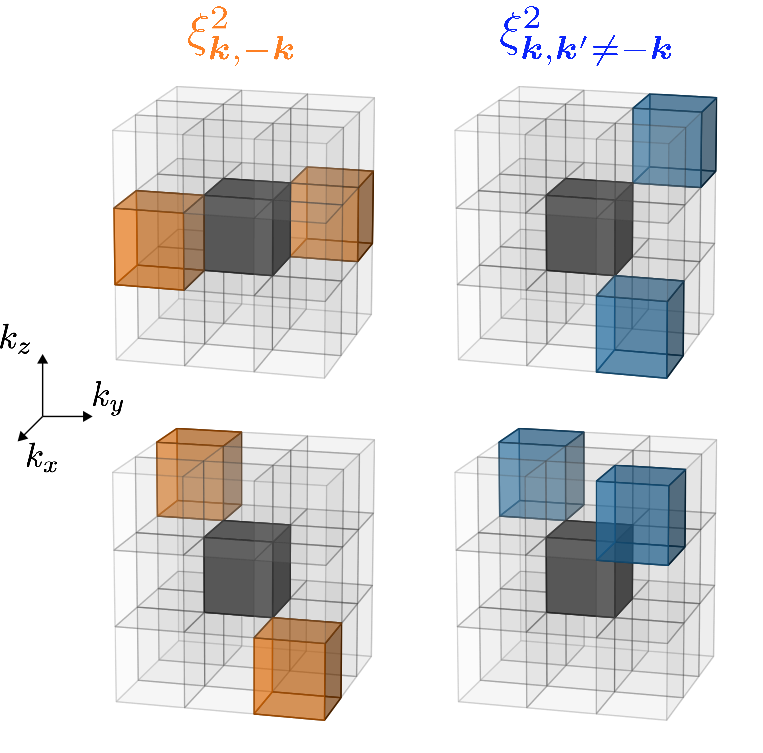
\includegraphics[width=0.7\textwidth]{Fig/Chapter4/squeezing.png}
    \caption{Relative number squeezing measurement. The number of detected atoms in cubic boxes are recorded for each experimental run. We compute the squeezing parameter $\xi$ between correlated (orange) boxes as illustrated on the right, or uncorrelated (blue) boxes on the left. The central black box corresponds to the BEC, removed from the analysis.}
    \label{fig:squeezing}
\end{figure}

The results are summarized in table \ref{tab:squeezing}. For the low-temperature, high condensed fraction data, we are indeed able to observe a small relative number squeezing within the errorbars. For uncorrelated modes, the squeezing parameter is very slightly above 1, highlighting that the correlations indeed reduce the fluctuations of the number difference. For higher temperatures (lower condensed fraction), no relative number squeezing is observed as the correlations are drowned out. In addition, we see that the squeezing parameter increases as we increase the temperature. This is due to global atom number fluctuations of the order of $30\%$ in our experiment. At low temperature, there are few detected atoms and the shot noise is thus large and dominating the total atom number fluctuations. On the opposite, at higher temperatures, the number of depleted atoms increases, reducing the shot noise. The contribution of total atom number fluctuations are then not negligible anymore and increase the fluctuations of the number difference, higher than what is expected for a Poisson law, explaining why we observe $\xi^2 > 1$.

\begin{table}[]
    \arrayrulecolor{black}
    \centering
    \begin{tabular}{|c|c|c|}
        \hline
        $f_c$ & $\xi^2_{\bm{k},-\bm{k}}$ & $\xi^2_{\bm{k},\bm{k}}$ \\
        \hline
        0.84 & 0.992(3) & 1.004(3) \\
        \hline
        0.55 & 1.017(4) & 1.017(3) \\
        \hline
        0.29 & 1.040(5) & 1.045(5) \\
        \hline
    \end{tabular}
    \caption{Experimental values of the squeezing parameter for correlated and uncorrelated modes and different condensed fractions.}
    \label{tab:squeezing}
\end{table}


\section{Study of the width of the correlation peaks}

The last aspect of the \kmk correlation signal that remains to be studied so far is the width of the correlation peak. Once again, this quantity contains meaningful information about the many-body ground state. The key aspect is the same used by Hanbury Brown and Twiss in their seminal paper to measure the size of Sirius through the measurement of the second order correlation function: the width of the correlation is inversely proportional to the spatial size of the source. 

As we have done throughout this chapter, we will compare the predictions for both anomalous and normal correlations. We then need to determine what are the sizes of the components responsible for both correlation signals. On the one hand, the anomalous correlations are exclusively caused by quantum depleted atoms. The quantum depletion is non-existent outside of the BEC so its spatial is the one of the BEC. Therefore, we expect the width of the anomalous correlation peak $\sigma_A$ to be inversely proportional to the size of the BEC $L_{\rm{BEC}}$. On the other hand, the normal correlations are caused by quantum depleted atoms but also and importantly thermally depleted atoms whose spatial size extends beyond the BEC because of the increased kinetic energy. This tells us that the width of the normal correlations peak $\sigma_N$ should be smaller than for anomalous correlations.

\begin{figure}
    \centering
    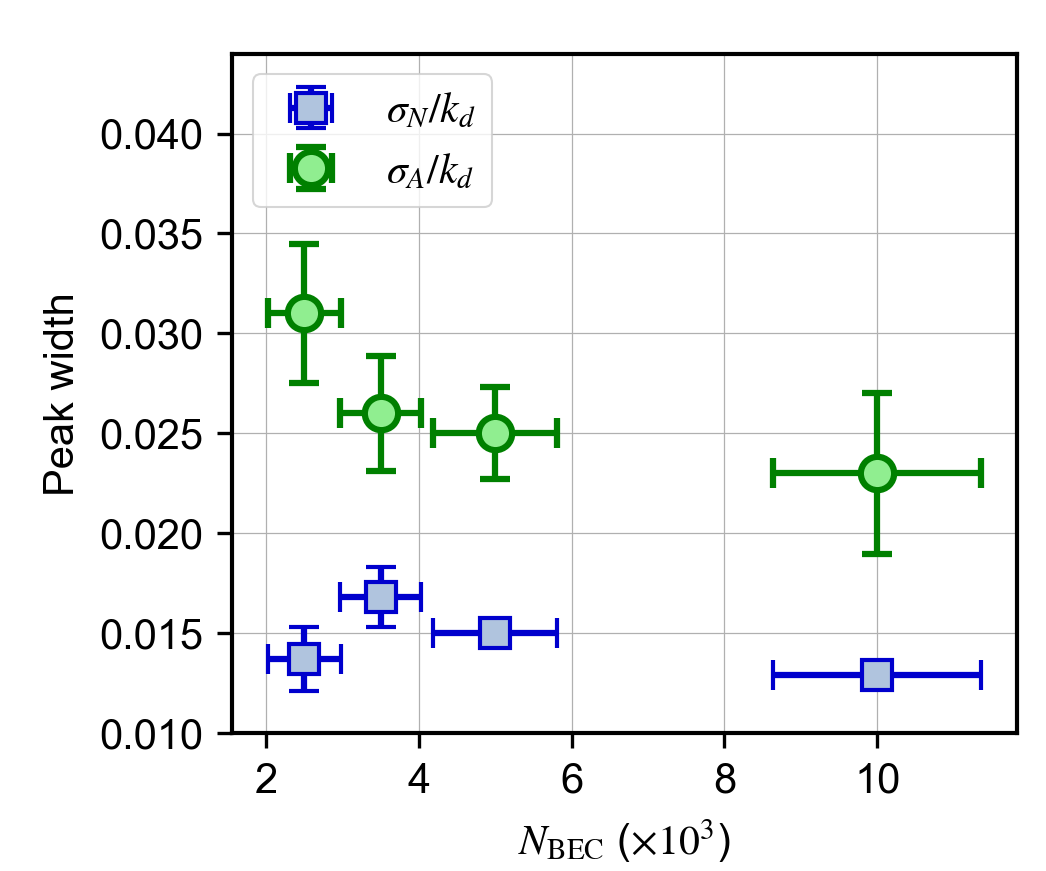
\includegraphics[width=0.65\textwidth]{Fig/Chapter4/width.png}
    \caption{Caption}
    \label{fig:width}
\end{figure}

We plot on Fig.-\ref{fig:width} the experimental correlation peaks widths for different total atom numbers. As expected, we observe that for all atom numbers, $\sigma_A > \sigma_N$. In addition, one would expect to see both widths decrease with the total atom number as the size of the system grows. This is more or less what the experimental data suggests but the error bar are not small enough to make a proper conclusion on this point. Note that in the Thomas-Fermi regime, the size of the BEC changes slowly with the total atom number $L_{\rm{BEC}} \propto \NBEC^{1/5}$ \NOTE{COMPLETER}

We now look at the quantitative value of $\sigma_A$ for which we have a theoretical prediction. This prediction has been obtained by S. Butera and I. Carusotto from the BEC center in Trento, Italy, applying the Bogoliubov theory for a trapped system. Their numerical calculations predict $\sigma_{A,\rm{theo}} = 0.94 \sigma_{\rm{BEC}}$, with $\sigma_{\rm{BEC}}$ the RMS width in momentum space of the condensante (\NOTE{REF}). 

To extract the value of $\sigma_{\rm{BEC}}$, we need to be careful of the saturation of the detector. Indeed, the BEC is very dense resulting in a high flux of atoms totally saturating the detector. If we plot 1D cuts of the momentum density, the BEC momentum profile is then flattened at the top and fitting with a Gaussian function over-evaluates the momentum width of the condensate. To circumvent this issue, we adapt the parameters of the Raman transfer (\NOTE{RAJOUTER SECTION}) to reduce drastically the detection efficiency and thus the flux of atoms to avoid saturation of the detector and ensure proper fitting.

During our first analysis, we noticed that the anomalous correlation peak was larger than the BEC, contrary to what we would have expected. We also noticed that the momentum width of the BEC was larger than what we obtained applying the Gutzwiller ansatz with our calibrated atom numbers. We attribute this to an imperfection in our experiment, the shot-to-shot fluctuations of the center-of-mass of the atomic distribution. When averaging over many experimental runs, these fluctuations enlarges artificially the measured width of the BEC, as well as the width of the anomalous correlation peak. These fluctuations are nevertheless easy to characterize by comparing the experimental momentum width of the BEC to the one predicted by the Gutzwiller variational approach.

When accounting for center-of-mass fluctuations, the measured momentum density results from the convolution with the distribution of center-of-mass displacements and has a RMS width:

\begin{equation}
    \sigma_{\rm{BEC}}=\sqrt{\sigma_{\rm{BEC},0}^2+\Delta k_{\rm{com}}^2}
\end{equation}

where $\sigma_{\rm{BEC},0}$ is the "true" BEC momentum width. The Gutzwiller variational approach gives  $\sigma_{\rm{BEC},0} \simeq 1.7 \times 10^{-2} \ k_d$ for a total atom number $\NBEC = 5 \times 10^5$ and we measure $\sigma_{\rm{BEC}}=2.0(1) \times 10^{-2} \ k_d$. From this we deduce $\Delta k_{\rm{com}}=1.1(1) \times 10^{-2} \ k_d$.

For a \kmk pair of atoms, a center-of-mass displacement ${\rm{d}} \bm{k}$ induces a momentum difference $\delta \bm{k}=2 {\rm{d}} \bm{k}$. The effect of the fluctuations are thus twice larger for anomalous correlations peak width than for the BEC momentum width:

\begin{equation}
    \sigma_A = \sqrt{\sigma_{A,0}^2+4\Delta k_{\rm{com}}^2}
\end{equation}

Injecting the theoretical prediction, we find that we should observe $\sigma_A \simeq 1.4(1) \sigma_{\rm BEC}$. This is consistent with our measurement, $\sigma_A = 1.2(1) \sigma_{\rm BEC}$.

\section{Conclusion}

\NOTE{TO DO}


